\fancyhead[L]{\small\textsf{\textbf{MỤC 1.5}\quad Hàm số ngược và Logarit}}
\fancyhead[R]{\small\textsf{\textbf{61}}}

\noindent
\begin{minipage}[t]{0.26\textwidth}
    \vspace{0pt}
    \centering
    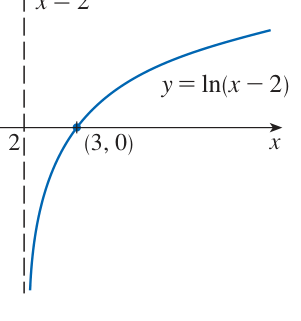
\includegraphics[width=\textwidth]{images/p0096_fig1.png}
    \vspace{2pt}
    \begin{flushleft}
        \textbf{\textsf{HÌNH 13}}\\
        {\small Đồ thị của hàm số $y = \ln x$ là hình phản xạ của đồ thị hàm số $y = e^x$ qua đường thẳng $y = x$.}
    \end{flushleft}

    \vspace{2.62cm}
    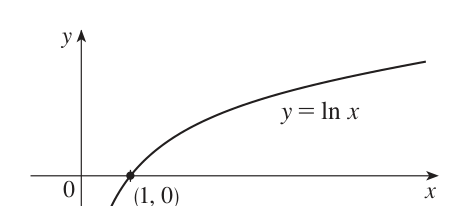
\includegraphics[width=\textwidth]{images/p0096_fig2.png}
    \vspace{2pt}
    \begin{flushleft}
        \textbf{\textsf{HÌNH 14}}
    \end{flushleft}
\end{minipage}%
\hfill
\begin{minipage}[t]{0.71\textwidth}
    \vspace{0pt}
    \noindent\textbf{\textsf{\color{stewartcyan}VÍ DỤ 11}}\quad Tính giá trị của $\log_8 5$ chính xác đến sáu chữ số thập phân.

    \vspace{0.25em}
    \noindent\textbf{\textsf{\color{stewartcyan}LỜI GIẢI}}\quad Công thức 11 cho ta
    \[
    \log_8 5 = \frac{\ln 5}{\ln 8} \approx 0{,}773976 \tag*{{\color{stewartcyan}$\blacksquare$}}
    \]

    \vspace{0.41em}
    \noindent{\color{stewartcyan}\rule{1.2ex}{1.2ex}}\hspace{0.5em}\textbf{\textsf{\large Đồ thị và sự tăng trưởng của hàm Logarit tự nhiên}}

    \vspace{0.33em}
    \noindent Đồ thị của hàm số mũ $y = e^x$ và hàm ngược của nó, hàm logarit tự nhiên, được thể hiện trong Hình 13. Tương tự như tất cả các hàm logarit khác với cơ số lớn hơn 1, logarit tự nhiên là một hàm tăng xác định trên $(0, \infty)$ và trục $y$ là tiệm cận đứng. (Điều này có nghĩa là các giá trị của $\ln x$ tiến tới âm vô cùng lớn khi $x$ dần tiến về 0.)

    \vspace{0.66em}
    \noindent\textbf{\textsf{\color{stewartcyan}VÍ DỤ 12}}\quad Vẽ phác thảo đồ thị của hàm số $y = \ln(x - 2) - 1$.

    \vspace{0.25em}
    \noindent\textbf{\textsf{\color{stewartcyan}LỜI GIẢI}}\quad Chúng ta bắt đầu từ đồ thị của $y = \ln x$ như đã cho ở Hình 13. Dựa vào các phép biến đổi đồ thị ở Mục 1.3, ta tịnh tiến đồ thị sang phải 2 đơn vị để nhận được đồ thị của hàm số $y = \ln(x - 2)$, sau đó tịnh tiến tiếp xuống dưới 1 đơn vị để nhận được đồ thị của $y = \ln(x - 2) - 1$. (Xem Hình 14.)

    \vspace{0.41em}
    \noindent
    \begin{minipage}[b]{0.48\textwidth}
        \centering
        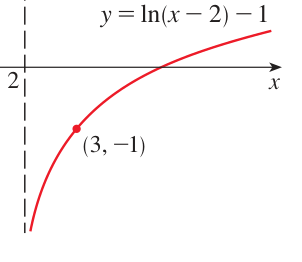
\includegraphics[width=\linewidth]{images/p0096_fig3.png}
    \end{minipage}\hfill
    \begin{minipage}[b]{0.48\textwidth}
        \centering
        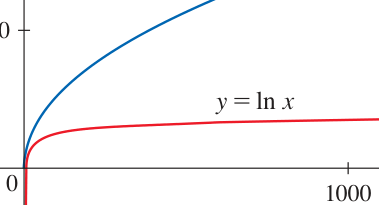
\includegraphics[width=\linewidth]{images/p0096_fig4.png}
    \end{minipage}
    \hfill{\color{stewartcyan}$\blacksquare$}

    \vspace{0.82em}
    \noindent Mặc dù $\ln x$ là một hàm tăng, nó tăng \textit{rất} chậm khi $x > 1$. Trên thực tế, $\ln x$ tăng chậm hơn bất kỳ lũy thừa dương nào của $x$. Để minh họa điều này, chúng tôi biểu diễn đồ thị của $y = \ln x$ và $y = x^{1/2} = \sqrt{x}$ trong các Hình 15 và 16. Bạn có thể thấy rằng ban đầu hai đồ thị tăng với tốc độ tương đối bằng nhau, nhưng cuối cùng hàm căn thức sẽ vượt xa hàm logarit.

    \vspace{0.66em}
    \noindent
    \begin{minipage}[t]{0.48\textwidth}
        \centering
        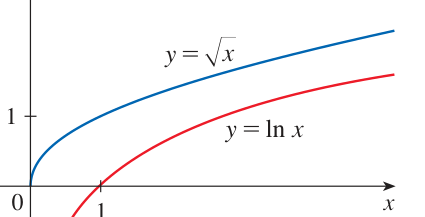
\includegraphics[width=\linewidth]{images/p0096_fig5.png}
        \vspace{2pt}
        \begin{flushleft}
            \textbf{\textsf{HÌNH 15}}
        \end{flushleft}
    \end{minipage}\hfill
    \begin{minipage}[t]{0.48\textwidth}
        \centering
        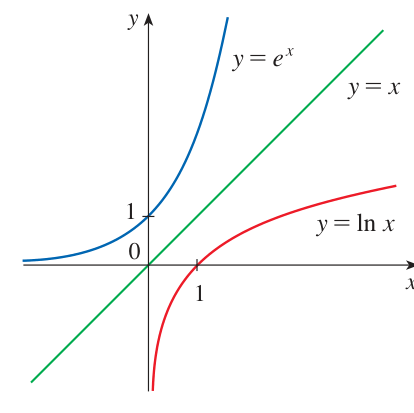
\includegraphics[width=\linewidth]{images/p0096_fig6.png}
        \vspace{2pt}
        \begin{flushleft}
            \textbf{\textsf{HÌNH 16}}
        \end{flushleft}
    \end{minipage}

    \vspace{0.66em}
    \noindent{\color{stewartcyan}\rule{1.2ex}{1.2ex}}\hspace{0.5em}\textbf{\textsf{\large Các hàm lượng giác ngược}}

    \vspace{0.33em}
    \noindent Khi chúng ta cố gắng tìm các hàm số lượng giác ngược, chúng ta sẽ gặp một trở ngại nhỏ: bởi vì các hàm lượng giác không phải là hàm một-đối-một (đơn ánh), nên chúng không có hàm ngược. Khó khăn này được khắc phục bằng cách thu hẹp miền xác định của các hàm số này lại để chúng trở thành các hàm một-đối-một.
\end{minipage}